% **************************************************************************************************
% ** SPSC Report and Thesis Template
% **************************************************************************************************
%
% ***** Authors *****
% Daniel Arnitz, Paul Meissner, Stefan Petrik
% Signal Processing and Speech Communication Laboratory (SPSC)
% Graz University of Technology (TU Graz), Austria
%
% ***** Changelog *****
% 0.1   2010-01-25   extracted from report template by Daniel Arnitz (not ready yet)
% 0.2   2010-02-08   added thesis titlepage and modified layout (not ready yet)
% 0.3   2010-02-18   added TUG logo and statutory declaration
% 0.4   2010-02-18   moved the information fields below % **************************************************************************************************
% ** SPSC Report and Thesis Template
% **************************************************************************************************
%
% ***** Authors *****
% Daniel Arnitz, Paul Meissner, Stefan Petrik
% Signal Processing and Speech Communication Laboratory (SPSC)
% Graz University of Technology (TU Graz), Austria
%
% ***** Changelog *****
%
% ***** Todo *****
%
% **************************************************************************************************



\documentclass[%
a4paper,% !!! ATTENTION: geometry package below !!!
\Twosided,% !!! ATTENTION: geometry package below !!!
openany,% begin chapters with new right page (openright) or don't care (openany)
11pt,%
fleqn,% equations not centered, but on the left side
tablecaptionbelow,% captions below tables
% titlepage,% use title
pointlessnumbers,% do not generate point at the end of section numbers (e.g. 1.4.5 instead of 1.4.5.)
final,%
]{scrreprt}% (KOMA)

\usepackage[paper=a4paper,\Twosided,%
textheight=246mm,%
textwidth=160mm,%
heightrounded=true,% round textheight to multiple of lines (avoids overfull vboxes)
ignoreall=true,% do not include header, footer, and margins in calculations
marginparsep=5pt,% marginpar only used for signs (centered), thus only small sep. needed
marginparwidth=10mm,% prevent margin notes to be out of page
hmarginratio=2:1,% set margin ration (inner:outer for twoside) - (2:3 is default)
]{geometry}%


% master
\usepackage{ifthen}% for optional parts
\usepackage[latin1]{inputenc}% German special characters
\ifthenelse{\equal{\DocumentLanguage}{en}}{\usepackage[USenglish]{babel}}{}%
\ifthenelse{\equal{\DocumentLanguage}{de}}{\usepackage[ngerman]{babel}}{}%
\usepackage[%
headtopline,plainheadtopline,% activate all lines (header and footer)
headsepline,plainheadsepline,%
footsepline,plainfootsepline,%
footbotline,plainfootbotline,%
automark% auto update \..mark
]{scrpage2}% (KOMA)
\usepackage{makeidx}% used to make an index directory
\usepackage[]{caption}% customize captions
\usepackage{multicol}%
\usepackage[stable,bottom,hang,splitrule,multiple,symbol*]{footmisc}% customize footnotes


% text
\usepackage{varioref}% improved references
\usepackage{color}% e.g., for color boxes
\usepackage{rotating}% to rotate objects
\usepackage{gensymb}% symbols (perthousand, Celsius, ...)
\usepackage[right]{eurosym}% euro symbol on the right side (51 EUR)
\usepackage[normalem]{ulem}% cross-out, strike-out, underlines (normalem: keep \emph italic)
%\usepackage[safe]{textcomp}% loading in safe mode to avoid problems (see LaTeX companion)
%\usepackage[geometry,misc]{ifsym}% technical symbols
\usepackage{remreset}%\@removefromreset commands (e.g., for continuous footnote numbering)
\usepackage[%
breaklinks=true,% allow line break in links
colorlinks=true,% if false: framed link
linkcolor=black,anchorcolor=black,citecolor=black,filecolor=black,%
menucolor=black,urlcolor=black]{hyperref}% hyperlinks for references


% math
\usepackage{amsmath,amssymb,amstext,bm} % use math packages
\usepackage{mathcomp}% symbols (perthousand, ...) in math mode


% graphics
\usepackage{graphicx}% use simple graphics
\usepackage{subfigure}% subfigures (a),(b),(c)... within figures
\usepackage{flafter}% place floats always after reference
\usepackage{placeins}% preventing floats from crossing a barrier
\usepackage{float}% to place floats !HERE!
\usepackage{psfrag}% replace text in eps figures


% tables
\usepackage{hhline}% hline doesn't work with colored columns, so using hhline
\usepackage{longtable}% for tables longer than one page
\usepackage{dcolumn}% for number alignment in tables
\usepackage{colortbl}% color in tables


% listings
%\usepackage{alltt}% verbatim environment with commands available
\usepackage{listings}% program code listings


% other
%\usepackage{layout}% graphical page layout (spacings)
\usepackage{xspace}% add space after macros if not followed by punctuation character
\makeindex% used for index creation

 (encoding...)
% 0.5   2010-03-02   added \ShortTitle to fix problems with long thesis titles
%                    added \ThesisType (makes the template suitable for MSc, BSc, PhD, ... Thesis)
%
% ***** Todo *****
% - Introduction/Usage
% **************************************************************************************************

% **************************************************************************************************
% basic setup
\newcommand{\DocumentType}{report} % "thesis" / "report"
\newcommand{\DocumentLanguage}{de} % "en" / "de"
\newcommand{\Twosided}{} % "twoside" / ""


% **************************************************************************************************
% template setup -- do not change these unless you know what you are doing!
% **************************************************************************************************
% ** SPSC Report and Thesis Template
% **************************************************************************************************
%
% ***** Authors *****
% Daniel Arnitz, Paul Meissner, Stefan Petrik
% Signal Processing and Speech Communication Laboratory (SPSC)
% Graz University of Technology (TU Graz), Austria
%
% ***** Changelog *****
%
% ***** Todo *****
%
% **************************************************************************************************



\documentclass[%
a4paper,% !!! ATTENTION: geometry package below !!!
\Twosided,% !!! ATTENTION: geometry package below !!!
openany,% begin chapters with new right page (openright) or don't care (openany)
11pt,%
fleqn,% equations not centered, but on the left side
tablecaptionbelow,% captions below tables
% titlepage,% use title
pointlessnumbers,% do not generate point at the end of section numbers (e.g. 1.4.5 instead of 1.4.5.)
final,%
]{scrreprt}% (KOMA)

\usepackage[paper=a4paper,\Twosided,%
textheight=246mm,%
textwidth=160mm,%
heightrounded=true,% round textheight to multiple of lines (avoids overfull vboxes)
ignoreall=true,% do not include header, footer, and margins in calculations
marginparsep=5pt,% marginpar only used for signs (centered), thus only small sep. needed
marginparwidth=10mm,% prevent margin notes to be out of page
hmarginratio=2:1,% set margin ration (inner:outer for twoside) - (2:3 is default)
]{geometry}%


% master
\usepackage{ifthen}% for optional parts
\usepackage[latin1]{inputenc}% German special characters
\ifthenelse{\equal{\DocumentLanguage}{en}}{\usepackage[USenglish]{babel}}{}%
\ifthenelse{\equal{\DocumentLanguage}{de}}{\usepackage[ngerman]{babel}}{}%
\usepackage[%
headtopline,plainheadtopline,% activate all lines (header and footer)
headsepline,plainheadsepline,%
footsepline,plainfootsepline,%
footbotline,plainfootbotline,%
automark% auto update \..mark
]{scrpage2}% (KOMA)
\usepackage{makeidx}% used to make an index directory
\usepackage[]{caption}% customize captions
\usepackage{multicol}%
\usepackage[stable,bottom,hang,splitrule,multiple,symbol*]{footmisc}% customize footnotes


% text
\usepackage{varioref}% improved references
\usepackage{color}% e.g., for color boxes
\usepackage{rotating}% to rotate objects
\usepackage{gensymb}% symbols (perthousand, Celsius, ...)
\usepackage[right]{eurosym}% euro symbol on the right side (51 EUR)
\usepackage[normalem]{ulem}% cross-out, strike-out, underlines (normalem: keep \emph italic)
%\usepackage[safe]{textcomp}% loading in safe mode to avoid problems (see LaTeX companion)
%\usepackage[geometry,misc]{ifsym}% technical symbols
\usepackage{remreset}%\@removefromreset commands (e.g., for continuous footnote numbering)
\usepackage[%
breaklinks=true,% allow line break in links
colorlinks=true,% if false: framed link
linkcolor=black,anchorcolor=black,citecolor=black,filecolor=black,%
menucolor=black,urlcolor=black]{hyperref}% hyperlinks for references


% math
\usepackage{amsmath,amssymb,amstext,bm} % use math packages
\usepackage{mathcomp}% symbols (perthousand, ...) in math mode


% graphics
\usepackage{graphicx}% use simple graphics
\usepackage{subfigure}% subfigures (a),(b),(c)... within figures
\usepackage{flafter}% place floats always after reference
\usepackage{placeins}% preventing floats from crossing a barrier
\usepackage{float}% to place floats !HERE!
\usepackage{psfrag}% replace text in eps figures


% tables
\usepackage{hhline}% hline doesn't work with colored columns, so using hhline
\usepackage{longtable}% for tables longer than one page
\usepackage{dcolumn}% for number alignment in tables
\usepackage{colortbl}% color in tables


% listings
%\usepackage{alltt}% verbatim environment with commands available
\usepackage{listings}% program code listings


% other
%\usepackage{layout}% graphical page layout (spacings)
\usepackage{xspace}% add space after macros if not followed by punctuation character
\makeindex% used for index creation


\input{./base/layout_\DocumentType}
% **************************************************************************************************
% ** SPSC Report and Thesis Template
% **************************************************************************************************
%
% ***** Authors *****
% Daniel Arnitz, Paul Meissner, Stefan Petrik
% Signal Processing and Speech Communication Laboratory (SPSC)
% Graz University of Technology (TU Graz), Austria
%
% ***** Changelog *****
%
% ***** Todo *****
%
% **************************************************************************************************



% **************************************************************************************************
% * SECTIONING AND TEXT
% **************************************************************************************************

% new chapter, section, ... plus a few addons
%   part
\newcommand{\newpart}[2]{\FloatBarrier\cleardoublepage\part{#1}\label{part:#2}}%
%   chapter
\newcommand{\newchapter}[2]{\FloatBarrier\chapter{#1}\label{chp:#2}}
\newcommand{\newchapterNoTOC}[2]{\FloatBarrier\stepcounter{chapter}\chapter*{#1}\label{chp:#2}}%
%   section
\newcommand{\newsection}[2]{\FloatBarrier\vspace{5mm}\section{#1}\label{sec:#2}}%
\newcommand{\newsectionNoTOC}[2]{\FloatBarrier\vspace{5mm}\stepcounter{section}\section*{#1}\label{sec:#2}}%
%   subsection
\newcommand{\newsubsection}[2]{\FloatBarrier\vspace{3mm}\subsection{#1}\label{sec:#2}}%
\newcommand{\newsubsectionNoTOC}[2]{\FloatBarrier\vspace{3mm}\stepcounter{subsection}\subsection*{#1}\label{sec:#2}}%
%   subsubsection
\newcommand{\newsubsubsection}[2]{\vspace{2mm}\subsubsection{#1}\label{sec:#2}}%
\newcommand{\newsubsubsectionNoTOC}[2]{\vspace{2mm}\stepcounter{subsubsection}\subsubsection*{#1}\label{sec:#2}}%

% next paragraph
\newcommand{\nxtpar}{\par\bigskip}

% "stylish" quotes on the right side
\newcommand{\openingquote}[2]{\hfill\parbox[t]{10cm}{\itshape\raggedleft{"#1"}\\\footnotesize -- #2}\nxtpar}%

% direct quotes
% \newenvironment{directquote}{\nxtpar\hrule}{\hrule}\hfill\litref{#1}{#2}}

% warnings and attention signs in marginpar
\newcommand{\MDanger}{\marginpar{\Huge\centering\fbox{\textbf{!}}}}%
\newcommand{\MAttention}{\marginpar{\Huge\centering\textbf{!}}}%
\newcommand{\MHint}{\marginpar{\Huge\centering\textbf{\checkmark}}}%
\newcommand{\MQuestion}{\marginpar{\Huge\centering\textbf{?}}}%

% same footnote number as last one
\newcommand{\lastfootnotemark}{\addtocounter{footnote}{-1}\footnotemark}%

% value-unit commands (for 457 kHz, etc)
\newcommand{\vu}[2]{\mbox{$#1\,\text{#2}$}} % "value~unit" ... prevents e.g. 456 \linebreak mV
\newcommand{\vuc}[3]{\mbox{$#1\,\text{#2}\;#3\,\%$}} % "value~unit~tolerance-per-cent"
\newcommand{\vum}[3]{\mbox{$#1\,\text{#2}\;#3\,\perthousand$}} % "value~unit~tolerance-per-mil"

% reminders
\newcommand{\reminder}[1]{\colorbox{red}{#1}\xspace}%
\newcommand{\rem}{\reminder{(...)}}%
\newcommand{\remq}{\reminder{???}}%
\newcommand{\uc}{\nxtpar\colorbox{yellow}{... under construction ...}\nxtpar}%

% misc
\newcommand{\pwd}{.} % present working directory (can be used to create relativ paths per part, etc.)


% **************************************************************************************************
% * MATH
% **************************************************************************************************

% highlighting
\newcommand{\vm}[1]{\bm{#1}}% vector or matrix

% operators
\newcommand{\E}[1]{\text{E}\!\left\{#1\right\}}% expectation operator
\newcommand{\var}[1]{\text{var}\!\left\{#1\right\}}% variance operator
\renewcommand{\ln}[1]{\text{ln}\!\left(#1\right)}% natural logarithm
\newcommand{\ld}[1]{\text{ld}\!\left(#1\right)}% logarithm base 2
\renewcommand{\log}[1]{\text{log}\!\left(#1\right)}% logarithm (base 10)
\newcommand{\logb}[2]{\text{log}_{#1}\!\left(#2\right)}% logarithm base ...
\newcommand{\avgvar}[1]{\overline{\text{var}}\!\left\{#1\right\}}% average variance operator
\renewcommand{\Re}[1]{\text{Re}\!\left\{#1\right\}}% real part
\renewcommand{\Im}[1]{\text{Im}\!\left\{#1\right\}}% imaginary part

% other
\newcommand{\conj}{^\ast}% conjugate complex
\newcommand{\mtx}[2]{\left[\begin{array}{#1}#2\end{array}\right]}%vector/matrix


% **************************************************************************************************
% * FLOATS (FIGURES, TABLES, LISTINGS, ...)
% **************************************************************************************************

% figures without frames
%   standard
\newcommand{\fig}[3]{\begin{figure}\centering\includegraphics[width=\textwidth]{#1}\caption{#2}\label{fig:#3}\end{figure}}%
%   with controllable parameters
\newcommand{\figc}[4]{\begin{figure}\centering\includegraphics[#1]{#2}\caption{#3}\label{fig:#4}\end{figure}}%
%   two subfigures
\newcommand{\twofig}[6]{\begin{figure}\centering%
\subfigure[#2]{\includegraphics[width=0.495\textwidth]{#1}}%
\subfigure[#4]{\includegraphics[width=0.495\textwidth]{#3}}%
\caption{#5}\label{fig:#6}\end{figure}}%
%   two subfigures and controllable parameters
\newcommand{\twofigc}[8]{\begin{figure}\centering%
\subfigure[#3]{\includegraphics[#1]{#2}}%
\subfigure[#6]{\includegraphics[#4]{#5}}%
\caption{#7}\label{fig:#8}\end{figure}}%

% framed figures
%   standard
\newcommand{\figf}[3]{\begin{figure}\centering\fbox{\includegraphics[width=\textwidth]{#1}}\caption{#2}\label{fig:#3}\end{figure}}%
%   with controllable parameters
\newcommand{\figcf}[4]{\begin{figure}\centering\fbox{\includegraphics[#1]{#2}}\caption{#3}\label{fig:#4}\end{figure}}%
%   two subfigures
\newcommand{\twofigf}[6]{\begin{figure}\centering%
\fbox{\subfigure[#2]{\includegraphics[width=0.495\textwidth]{#1}}}%
\fbox{\subfigure[#4]{\includegraphics[width=0.495\textwidth]{#3}}}%
\caption{#5}\label{fig:#6}\end{figure}}%
%   two subfigures and controllable parameters
\newcommand{\twofigcf}[8]{\begin{figure}\centering%
\fbox{\subfigure[#3]{\includegraphics[#1]{#2}}}%
\fbox{\subfigure[#6]{\includegraphics[#4]{#5}}}%
\caption{#7}\label{fig:#8}\end{figure}}%

% listings
\newcommand{\filelisting}[4]{\lstinputlisting[print=true,language=#1,caption={#3},label={lst:#4}]{#2}}

% preserve backslash for linebreaks in tables (ragged... redefines \\, thus it has to be preserved)
\newcommand{\pbs}[1]{\let\temp=\\#1\let\\=\temp}%

\graphicspath{{./drawings/}{./plots/}{./images/}}
% **************************************************************************************************
% ATTENTION: Make sure that makeindex is set to -s "./base/index.sty"
% **************************************************************************************************

% uncomment to get watermarks:
% \usepackage[first,bottom,light,draft]{draftcopy}
% \draftcopyName{ENTWURF}{160}


% **************************************************************************************************
% information fields

% general
\newcommand{\DocumentTitle}{Adaptive Systems}
\newcommand{\DocumentSubtitle}{Assignment 1}
\newcommand{\ShortTitle}{Assignment 1} % used in headers (keep short!)
\newcommand{\DocumentAuthor}{Ebner Thomas (0831246), N�hmer Stefan (0830668)}
\newcommand{\DocumentDate}{Graz, \today}
%    for thesis only (will be ignored for reports)
\newcommand{\ThesisType}{Master's Thesis}
\newcommand{\Organizations}{Signal Processing and Speech Communications Laboratory \\ Graz University of Technology \\[1cm] on behalf of \\ Some Company} % SPSC \\ TUG \\[1cm] on behalf of \\ A Nice Company
\newcommand{\Advisors}{Dipl.-Ing. Dr. Assoc.Prof. Klaus Witrisal \\ Dipl.-Ing. Paul Meissner} % Advisor 1 \\ Advisor 2 \\ ...
\newcommand{\Supervisors}{Univ.-Prof. Dipl.-Ing. Dr.techn. Gernot Kubin}

% revision number
\newcommand{\RevPrefix}{alpha~}
\newcommand{\RevLarge}{1}
\newcommand{\RevSmall}{0}

% confidential?
\newcommand{\ConfidNote}{do not blend}% {"confidential", "eyes only", ...}





\begin{document}

%listingstyle:
\definecolor{orange}{rgb}{0.75,0.65,0}
\definecolor{gruen}{rgb}{0,0.5,0}
\definecolor{listinggray}{gray}{0.97}
\definecolor{listingshadow}{gray}{0.2}
\lstloadlanguages{Matlab}
\lstset{frame=shadowbox,
		rulesepcolor=\color{listingshadow},
		numbers=left,
		basicstyle=\scriptsize\ttfamily,
		numberstyle=\tiny,
		keywordstyle=\color{blue}\bfseries, % bold black keywords
		identifierstyle=, % nothing happens
		commentstyle=\color{gruen}, % comments
		stringstyle=\color{orange}, % typewriter type for strings
		showstringspaces=false,
		tabsize=4,
		backgroundcolor=\color{listinggray}
        }




% **************************************************************************************************
% titlepage
\input{./base/titlepage_\DocumentType}

% statutory declaration for theses
\ifthenelse{\equal{\DocumentType}{thesis}}{% **************************************************************************************************
% ** SPSC Report and Thesis Template
% **************************************************************************************************
%
% ***** Authors *****
% Daniel Arnitz, Paul Meissner, Andreas Laesser, Stefan Petrik
% Signal Processing and Speech Communication Laboratory (SPSC)
% Graz University of Technology (TU Graz), Austria
%
% ***** Changelog *****
% 0.1   2010-02-18   created
% 0.2   2010-03-02   added German declaration
%
% ***** Todo *****
% **************************************************************************************************

\cleardoublepage
\pagestyle{empty}\pagenumbering{roman}

\vspace*{1cm}

% English
\ifthenelse{\equal{\DocumentLanguage}{en}}{
\begin{center}\Large\bfseries Statutory Declaration\end{center}\vspace*{1cm}
\noindent I declare that I have authored this thesis independently, that I have not used other than the declared sources$/$resources, and that I have explicitly marked all material which has been quoted either literally or by content from the used sources.
\par\vspace*{4cm}
\centerline{
\begin{tabular}{m{1.5cm}cm{1.5cm}m{3cm}m{1.5cm}cm{1.5cm}}
\cline{1-3} \cline{5-7}
 & date & & & & (signature) &\\
\end{tabular}}
}

% German
\ifthenelse{\equal{\DocumentLanguage}{de}}{
\begin{center}\Large\bfseries Eidesstattliche Erkl�rung\end{center}\vspace*{1cm}
Ich erkl�re an Eides statt, dass ich die vorliegende Arbeit selbstst�ndig verfasst, andere als die angegebenen Quellen$/$Hilfsmittel nicht benutzt, und die den benutzten Quellen w�rtlich und inhaltlich entnommene Stellen als solche kenntlich gemacht habe.
\par\vspace*{4cm}
\centerline{
\begin{tabular}{m{1.5cm}cm{1.5cm}m{3cm}m{1.5cm}cm{1.5cm}}
\cline{1-3} \cline{5-7}
 & Graz, am & & & & (Unterschrift) &\\
\end{tabular}}
}

}{}


% **************************************************************************************************
% **************************************************************************************************
% user-defined part

\chapter{Analytic Problem 1.1}

\subsection{(a)}
Zuerst stellen wir eine Kostenfunktion $J(c)$, wie in den Problem-classes auf.

\begin{equation}
 J(c) = E\{e[n] \cdot e[n]\}
\end{equation}

Um das Minimum der Kostenfunktion zu ermitteln, bilden wir den Gradienten mit den Ableitungen nach den
einzelnen Filterkoeffizienten $\textbf{c}$.

\begin{equation}
 \bigtriangledown J(c) = E\{\bigtriangledown e[n] \cdot e[n]\}
 \label{eq:kosten1}
\end{equation}

Setzt man die Beziehung $e[n] = d[n] - \textbf{c}^T \textbf{x}[n]$ in die Gleichung \ref{eq:kosten1} ein,
so erh�lt man:

\begin{equation}
 \bigtriangledown J(c) = E\{(\bigtriangledown d[n] - \bigtriangledown \textbf{c}^T \textbf{x}[n]) \cdot e[n]\}
\end{equation}

\begin{equation}
 \bigtriangledown J(c) = E\{-\textbf{x}[n] \cdot e[n]\}
\end{equation}

Um nun das Minimum der Kostenfunktion zu erhalten m�ssen wir diesen Term 0 setzen:

\begin{equation}
 \bigtriangledown J(c) = E\{-\textbf{x}[n] \cdot e[n]\} \stackrel{!}{=} 0
 \label{eq:aresult}
\end{equation}

Hiermit ist ersichtlich, dass jedes $x[n-k]$ orthogonal zu $e[n]$ ist.


\subsection{(b)}

Um diese Beziehung herzuleiten verwenden wir die Gleichung \ref{eq:aresult} und multiplizieren
dise von links mit $\textbf{c}^T$.
Somit erhalten wir:

\begin{equation}
 E\{-\textbf{c}^T \textbf{x}[n] \cdot e[n]\} \stackrel{!}{=} 0
\end{equation}

\begin{equation}
 E\{-y[n] \cdot e[n]\} \stackrel{!}{=} 0
\end{equation}

Somit ist auch $y[n]$ orthogonal zu $e[n]$


\subsection{(c)}

Um den Wert f�r die Kostenfunktion bei optimalen Filterkoeffizienten zu berechnen, setzen wir einfach
die Wiener Hopf Solution in die Gleichung f�r die Kostenfunktion (Gleichung \ref{eq:kosten2}).

\begin{equation}
 J(\textbf{c}) = E\{d^2[n] - 2d[n]\textbf{c}^T\textbf{x}[n] + \textbf{c}^T\textbf{x}[n]\textbf{x}^T[n]\}
\end{equation}

\begin{equation}
 J(\textbf{c}) = E\{d^2[n]\} - 2\textbf{c}^T\textbf{p} + \textbf{c}^T\textbf{R}_{xx}
 \label{eq:kosten2}
\end{equation}

Somit erhalten wir:

\begin{equation}
 J(\textbf{c}) = \sigma_d - 2\textbf{p}^T\textbf{R}_{xx}\textbf{p} + \textbf{p}^T\textbf{R}_{xx}\textbf{p}
\end{equation}

\begin{equation}
 J(\textbf{c}) = \sigma_d - \textbf{p}^T\textbf{R}_{xx}\textbf{p}
\end{equation}
\clearpage
\chapter{Analytic Problem 1.2}

\subsection{(a) Berechnung von $\underline{c}_{MSE}$}
Zur Bestimmung von $\underline{c}_{MSE}$ muss zuerst eine Kostenfunktion $J(\underline{c})$ aufgestellt werden. Diese wird dann abgeleitet und eine Nullstelle gesucht (Suche nach dem Minimum). Dadurch erhält man $\underline{c}_{MSE}$, bei dem die Abweichung am geringsten ist. $x[n]$ und $\nu [n]$ sind dabei \emph{jointly stationary}.

\begin{equation}
  d[n] = \underline{h}^T \underline{x}[n] + \nu [n]
\end{equation}

\begin{equation}
 e[n] = d[n] - y[n] = \underline{h}^T \underline{x}[n] + \nu [n] - \underline{c}^T \underline{x}[n]
\end{equation}

Die Kostenfunktion ergibt sich zu:
\begin{eqnarray}
 J(\underline{c}) & = & E\{e^2[n]\} = E\{(\underline{h}^T \underline{x}[n] + \nu [n] - \underline{c}^T \underline{x}[n])^2\} \\
 & = & E\{\underline{h}^T \underline{x}[n] \underline{x}^T[n] \underline{h} + \nu [n] \underline{h}^T \underline{x}[n] - \underbrace{\underline{h}^T \underline{x}[n] \underline{x}^T[n] \underline{c}}_{\underline{c}^T \underline{x}[n] \underline{x}^T[n] \underline{h}} + \nu [n] \underline{h}^T \underline{x}[n] + \nu^2[n] \\
 & & - \nu [n] \underline{c}^T \underline{x}[n] - \underline{c}^T \underline{x}[n] \underline{x}^T[n] \underline{h} - \nu [n] \underline{c}^T \underline{x}[n] + \underline{c}^T \underline{x}[n] \underline{x}^T[n] \underline{c}\} \\
 & = & \underline{h}^T \underbrace{E\{\underline{x}[n] \underline{x}^T[n]\}}_{\underline{R}_{xx}} \underline{h} + 2 \underline{h}^T \underbrace{E\{\nu [n] \underline{x}[n]\}}_{0} - 2 \underline{c}^T \underbrace{E\{\underline{x}[n] \underline{x}^T[n]\}}_{\underline{R}_{xx}} \underline{h} + \underbrace{E\{\nu^2[n]\}}_{\sigma_\nu^2} \\
 & & - 2 \underline{c}^T \underbrace{E\{\nu [n] \underline{x}[n]\}}_{0} + \underline{c}^T \underbrace{E\{\underline{x}[n] \underline{x}^T[n]\}}_{\underline{R}_{xx}} \underline{c} \\
 & = & \underline{h}^T \underline{R}_{xx} \underline{h} - 2 \underline{c}^T \underline{R}_{xx} \underline{h} + \underline{c}^T \underline{R}_{xx} \underline{c} + \sigma_\mu^2
\end{eqnarray}

Diese wird abgeleitet:
\begin{equation}
 \underline{\bigtriangledown}_{\underline{c}_{MSE}} J(\underline{c}_{MSE}) = 0 - 2 \underline{R}_{xx} \underline{h} + 2 \underline{R}_{xx} \underline{c}_{MSE} + 0 \stackrel{!}{=} 0
\end{equation}

Daraus ergibt sich:
\begin{equation}
 \underline{R}_{xx} \underline{h} = \underline{R}_{xx} \underline{c}_{MSE} \Rightarrow \underline{c}_{MSE} = \underline{h}
\end{equation}

Vorraussetzung ist dabei, dass $\underline{R}_{xx}^{-1}$ existiert.

\subsection{(b) MMSE}

\begin{equation}
 J(\underline{c}_{MSE}) = \underline{h}^T \underline{R}_{xx} \underline{h} - 2 \underline{h}^T \underline{R}_{xx} \underline{h} + \underline{h}^T \underline{R}_{xx} \underline{h} + \sigma_\mu^2 = \sigma_\mu^2
\end{equation}


\subsection{(c) Bestimmung von $\underline{c}_{MSE}$ für bekanntes $\underline{h}$}

Bei der Bestimmung von $\underline{c}_{MSE}$ müssen die 3 unterschiedlichen Fälle betrachtet werden: $N<N_h$, $N=N_h$ und $N>N_h$.


\subsubsection{N=2}

In diesem Fall muss die Berechnung erneut gemacht werden, diesmal aber mit aufgeteilten Vektoren:

$$ \underline{x}'[n] = \begin{bmatrix} \underline{x}_a[n] \\ \underline{x}_b[n] \end{bmatrix} $$

Die Grösse des Vektors $\underline{x}[n]$ ist $(N_h,1)$, Teilvektor $\underline{x}_a[n]$ ist $(N,1)$, Teilvektor $\underline{x}_b[n]$ ist $(N_h-N,1)$.

\begin{equation}
  d[n] = \underbrace{\underline{h}^T}_{(1,N_h)} \underbrace{\underline{x}[n]}_{(N_h,1)} + \nu [n]
\end{equation}

\begin{equation}
  y[n] = \underbrace{\underline{c}^T}_{(1,N)} \underbrace{\underline{x}_a[n]}_{(N,1)}
\end{equation}

\begin{equation}
 e[n] = d[n] - y[n] = \underline{h}^T \underline{x}[n] + \nu [n] - \underline{c}^T \underline{x}_a[n]
\end{equation}

Man kann jetzt neue Korrelationsmatrizen definieren:

\begin{equation}
 E\{\underline{x}[n] \underline{x}^T[n]\} = E\{\begin{bmatrix} \underline{x}_a[n] \\ \underline{x}_b[n] \end{bmatrix} \begin{bmatrix} \underline{x}_a[n] & \underline{x}_b[n] \end{bmatrix}\} = E\{\begin{bmatrix} \underline{x}_a[n] \underline{x}_a^T[n] & \underline{x}_a[n] \underline{x}_b^T[n] \\ \underline{x}_b[n] \underline{x}_a^T[n] & \underline{x}_b[n] \underline{x}_b^T[n] \end{bmatrix}\} = \begin{bmatrix} \underline{R}_{aa} & \underline{R}_{ab} \\ \underline{R}_{ba} & \underline{R}_{bb} \end{bmatrix}
\end{equation}

\begin{equation}
 E\{\underline{x}[n] \underline{x}_a^T[n]\} = E\{\begin{bmatrix} \underline{x}_a[n] \\ \underline{x}_b[n] \end{bmatrix} \underline{x}_a[n]\} = E\{\begin{bmatrix} \underline{x}_a[n] \underline{x}_a^T[n] \\ \underline{x}_a[n] \underline{x}_a^T[n] \end{bmatrix} \} = \begin{bmatrix} \underline{R}_{aa} \\ \underline{R}_{ba} \end{bmatrix}
\end{equation}

\begin{equation}
 E\{\underline{x}_a[n] \underline{x}^T[n]\} = E\{\underline{x}_a[n] \begin{bmatrix} \underline{x}_a^T[n] & \underline{x}_b^T[n] \end{bmatrix}\} = E\{\begin{bmatrix} \underline{x}_a[n] \underline{x}_a^T[n] \\ \underline{x}_a[n] \underline{x}_b^T[n] \end{bmatrix}\} = \begin{bmatrix} \underline{R}_{aa} & \underline{R}_{ab} \end{bmatrix}
\end{equation}


Die Kostenfunktion ergibt sich für dieses Beispiel zu:
\begin{eqnarray}
 J(\underline{c}) & = & E\{e^2[n]\} = E\{(\underline{h}^T \underline{x}[n] + \nu [n] - \underline{c}^T \underline{x}_a[n])^2\} \\
 & = & E\{\underline{h}^T \underline{x}[n] \underline{x}^T[n] \underline{h} + \nu [n] \underline{h}^T \underline{x}[n] - \underbrace{\underline{h}^T \underline{x}[n] \underline{x}_a^T[n] \underline{c}}_{\underline{c}^T \underline{x}_a[n] \underline{x}^T[n] \underline{h}} + \nu [n] \underline{h}^T \underline{x}[n] + \nu^2[n] \\
 & & - \nu [n] \underline{c}^T \underline{x}_a[n] - \underline{c}^T \underline{x}_a[n] \underline{x}^T[n] \underline{h} - \nu [n] \underline{c}^T \underline{x}_a[n] + \underline{c}^T \underline{x}_a[n] \underline{x}_a^T[n] \underline{c}\} \\
 & = & \underline{h}^T E\{\underline{x}[n] \underline{x}^T[n]\} \underline{h} + 2 \underline{h}^T \underbrace{E\{\nu [n] \underline{x}[n]\}}_{0} - 2 \underline{c}^T E\{\underline{x}_a[n] \underline{x}^T[n]\} \underline{h} + \underbrace{E\{\nu^2[n]\}}_{\sigma_\nu^2} \\
 & & - 2 \underline{c}^T \underbrace{E\{\nu [n] \underline{x}_a[n]\}}_{0} + \underline{c}^T E\{\underline{x}_a[n] \underline{x}_a^T[n]\} \underline{c} \\
 & = & \underline{h}^T \underline{R}_{xx} \underline{h} - 2 \underline{c}^T [ \underline{R}_{aa} \underline{R}_{ab} ] \underline{h} + \underline{c}^T \underline{R}_{aa} \underline{c} + \sigma_\mu^2
\end{eqnarray}

Die Kostenfunktion wird wieder abgeleitet und 0 gesetzt:
\begin{equation}
 \underline{\bigtriangledown}_{\underline{c}_{MSE}} J(\underline{c}_{MSE}) = 0 + 0 - 2 \begin{bmatrix} \underline{R}_{aa} & \underline{R}_{ab} \end{bmatrix} \underline{h} + 2 \underline{R}_{xx} \underline{c}_{MSE} + 0 \stackrel{!}{=} 0
\end{equation}

Daraus ergibt sich:
\begin{equation}
 \begin{bmatrix} \underline{R}_{aa} & \underline{R}_{ab} \end{bmatrix} \begin{bmatrix} \underline{h}_a \\ \underline{h}_b \end{bmatrix} = \underline{R}_{aa} \underline{c}_{MSE} \Rightarrow \underline{c}_{MSE} = \underline{R}_{aa}^{-1} (\underline{R}_{aa} \underline{h}_a + \underline{R}_{ab} \underline{h}_b ) = \underline{h}_a \underline{R}_{aa}^{-1} \underline{R}_{ab} \underline{h}_b )
\end{equation}

Da $x[n]$ ein \emph{white, zero-mean} Signal ist, gilt $ E\{x[n] x[n-k]\} = 0 \forall k $, d.h. $\underline{R}_{xx}$ ist eine Diagonalmatrix, wobei alle Elemente in der Diagonale den Wert $\sigma_x^2$, also $\underline{R}_{xx} = \underline{I} \sigma_x^2$. Dadurch ergibt sich auch, dass $\underline{R}_{ab} = \underline{R}_{ba} = \underline{0}$. Dadurch ergibt sich:

\begin{equation}
 \underline{c}_{MSE} = \underline{h}_a \underline{R}_{aa}^{-1} \underline{0} \underline{h}_b = \underline{h}_a = \begin{bmatrix} 1 \\ -1 \end{bmatrix}
\end{equation}

Der MMSE berechnet sich zu:
\begin{eqnarray}
 J(\underline{c}_{MSE}) & = & \underline{h}^T \underline{R}_{xx} \underline{h} - 2 \underline{h}_a^T \begin{bmatrix} \underline{R}_{aa} & \underline{R}_{ab} \end{bmatrix} \underline{h} + \underline{h}_a^T \underline{R}_{aa} \underline{h}_a + \sigma_\mu^2 \\
 & = & \begin{bmatrix} \underline{h}_a^T & \underline{h}_b^T \end{bmatrix} \begin{bmatrix} \underline{R}_{aa} & \underline{R}_{ab} \\ \underline{R}_{ba} & \underline{R}_{bb} \end{bmatrix} \begin{bmatrix} \underline{h}_a \\ \underline{h}_b \end{bmatrix}  - 2 \underline{h}_a^T \begin{bmatrix} \underline{R}_{aa} & \underline{R}_{ab} \end{bmatrix} \begin{bmatrix} \underline{h}_a \\ \underline{h}_b \end{bmatrix} + \underline{h}_a^T \underline{R}_{aa} \underline{h}_a + \sigma_\mu^2 \\
 & = & \underline{h}_a^T \underline{R}_{aa} \underline{h}_a + \underline{h}_a^T \underline{R}_{ab} \underline{h}_b + \underline{h}_b^T \underline{R}_{ba} \underline{h}_a + \underline{h}_b^T \underline{R}_{bb} \underline{h}_b - 2 \underline{h}_a^T \underline{R}_{aa} \underline{h}_a \\
 & & - 2 \underline{h}_a^T \underline{R}_{ab} \underline{h}_b + \underline{h}_a^T \underline{R}_{aa} \underline{h}_a + \sigma_\nu^2 \\
 & = & - \underline{h}_a^T \underline{R}_{ab} \underline{h}_b + \underline{h}_b^T \underline{R}_{ba} \underline{h}_a + \underline{h}_b^T \underline{R}_{bb} \underline{h}_b + \sigma_\nu^2
\end{eqnarray}

Da $\underline{R}_{ab} = \underline{R}_{ba} = \underline{0}$ ergibt sich:
\begin{equation}
 MMSE = - \underline{h}_a^T \underline{0} \underline{h}_b + \underline{h}_b^T \underline{0} \underline{h}_a + \underline{h}_b^T \underline{R}_{bb} \underline{h}_b + \sigma_\nu^2 = \underline{h}_b^T \underline{R}_{bb} \underline{h}_b + \sigma_\nu^2
\end{equation}

Mit $\underline{h}_b = 1$ (das letzte Element von $\underline{h}$ und $\underline{R}_{bb} = 1$ (das rechte untere Element von $\underline{R}_{xx}$, also $\sigma_x^2 = 1$) erhält man für den MMSE:
\begin{equation}
 MMSE = 1 \cdot 1 \cdot 1 + 0.5 = 1.5
\end{equation}

Das adaptive System hat eine geringere Ordnung als das unbekannte System, es ist also ``unterbestimmt''. Wie in den Problem Classes erklärt kann ein adaptives System einer geringeren Ordnung als das unbekannte System dieses nicht richtig abbilden, dadurch steigt der Fehler (und auch der MMSE).

\subsubsection{N=3}

Dies ist der einfache Fall mit $N=N_h$, die mit der Gleichung aus Aufgabe (a) berechnet werden kann.

\begin{equation}
 \underline{c}_{MSE} = \underline{h} = \begin{bmatrix} 1 \\ -1 \\ 1 \end{bmatrix}
\end{equation}

\begin{equation}
 MMSE = \sigma_\nu^2 = 0.5
\end{equation}

In diesem Fall ist die Ordnung des adaptiven Systems gleich der Ordnung des unbekannten Systems. Es kann also gut abgebildet werden, und der Fehler wird minimiert. Der MMSE entspricht der Rauschleistung des Eingangsrauschens.


\subsubsection{N=4}

Dieser Fall (überbestimmt) ist auch einfach zu lösen. Wie in den Problem Classes gezeigt können die Vektoren mit 0 aufgefüllt werden:

$$ \underline{h}' = \begin{bmatrix} 1 \\ -1 \\ 1 \\ 0 \end{bmatrix}, \underline{x}'[n] = \begin{bmatrix} \underline{x}[n] \\ 0 \end{bmatrix} $$

\begin{equation}
 \underline{c}_{MSE} = \underline{h} = \begin{bmatrix} 1 \\ -1 \\ 1 \end{bmatrix}
\end{equation}

\begin{equation}
 MMSE = \sigma_\nu^2 = 0.5
\end{equation}

In diesem Fall ist die Ordnung des adaptiven Systems grösser als die Ordnung des unbekannten Systems. Deswegen kann es auch wieder gut abgebildet werden und der Fehler wird minimal (wie im Fall $N=N_h$).


\subsection{(d) Berechnung der Korrelationsvektoren von $\nu$}

Aus der Definition von $r_{\nu x}$ erhält man:
\begin{equation}
 r_{\nu x}[k] = E\{\nu[n] x[n-k]\} = E\{\frac{1}{2} (x[n] + x[n-1]) x[n-k]\} = \frac{1}{2} E\{x[n] x[n-k]\} + \frac{1}{2} E\{x[n-1] x[n-k]\}
\end{equation}

Da $x[n]$ ein \emph{zero-mean, white gaussian noise} ist, gilt: $ r_{xx}[0] = \sigma_x^2 = 1, r_{xx}[k] = 0 \forall k \neq 0$. Betrachten wir die möglichen Fälle:

\begin{equation}
 k=0: r_{\nu x}[0] = \frac{1}{2} E\{x[n] x[n]\} + \frac{1}{2} E\{x[n-1] x[n]\} = \frac{1}{2} r_{xx}[0] + \frac{1}{2} r_{xx}[1] = \frac{1}{2}
\end{equation}

\begin{equation}
 k=1: r_{\nu x}[1] = \frac{1}{2} E\{x[n] x[n-1]\} + \frac{1}{2} E\{x[n-1] x[n-1]\} = \frac{1}{2} r_{xx}[1] + \frac{1}{2} r_{xx}[0] = \frac{1}{2}
\end{equation}

\begin{equation}
 k \geq 2: r_{\nu x}[k] = \frac{1}{2} E\{x[n] x[n-k]\} + \frac{1}{2} E\{x[n-1] x[n-k]\} = \frac{1}{2} r_{xx}[k] + \frac{1}{2} r_{xx}[k-1] = 0
\end{equation}

Für $r_{\nu \nu}$ ergibt sich:

\begin{eqnarray}
 r_{\nu \nu}[k] & = & E\{\nu[n] \nu[n-k]\} = E\{\frac{1}{2} (x[n] + x[n-1]) \frac{1}{2} (x[n-k] + x[n-k-1])\} \\
 & = & \frac{1}{4} E\{x[n] + x[n-k]\} + \frac{1}{4} E\{x[n] + x[n-k-1]\} \\
 & & + \frac{1}{4} E\{x[n-1] + x[n-k]\} + \frac{1}{4} E\{x[n-1] + x[n-k-1]\} \\
 & = & \frac{1}{4} r_{xx}[k] + \frac{1}{4} r_{xx}[k+1] + \frac{1}{4} r_{xx}[k-1] + \frac{1}{4} r_{xx}[k]
\end{eqnarray}

Wir unterscheiden wieder die möglichen Fälle:
\begin{equation}
 k=0: r_{\nu \nu}[0] = \frac{1}{4} r_{xx}[0] + \frac{1}{4} r_{xx}[1] + \frac{1}{4} r_{xx}[-1] + \frac{1}{4} r_{xx}[0] = \frac{1}{2}
\end{equation}

\begin{equation}
 k=1: r_{\nu \nu}[1] = \frac{1}{4} r_{xx}[1] + \frac{1}{4} r_{xx}[2] + \frac{1}{4} r_{xx}[0] + \frac{1}{4} r_{xx}[1] = \frac{1}{4}
\end{equation}

\begin{equation}
 k \geq 2: r_{\nu \nu}[2] = \frac{1}{4} r_{xx}[k] + \frac{1}{4} r_{xx}[k+1] + \frac{1}{4} r_{xx}[k-1] + \frac{1}{4} r_{xx}[k] = 0
\end{equation}

Für die Varianz $\sigma_\nu^2$ erhält man mit $\sigma_x^2 = 1$:
\begin{eqnarray}
 \sigma_\nu^2 & = & E\{\nu^2[n]\} = E\{\frac{1}{2} (x[n] + x[n-1]) \frac{1}{2} (x[n] + x[n-1])\} \\
 & = & \frac{1}{4} E\{x^2[n] + 2 x[n]x[n-1] + x^2[n-1]\} \\
 & = & \frac{1}{4} E\{x^2[n]\} + 2 \frac{1}{4} E\{x[n]x[n-1]\} + \frac{1}{4} E\{x^2[n-1]\} \\
 & = & \frac{1}{4} \sigma_x^2 + \frac{1}{2} r_{xx}[1] + \frac{1}{4} \sigma_x^2 = \frac{1}{4} 1 + \frac{1}{2} 0 + \frac{1}{4} 1 = \frac{1}{2}
\end{eqnarray}


\subsection{(e) $\underline{c}_{MSE}$ für nicht unkorrelierte $x$ und $\nu$}

Es müssen wieder neue Funktionen definiert werden:
\begin{equation}
  d[n] = \underline{h}^T \underline{x}[n] + \frac{1}{2} (x[n] + x[n-1])
\end{equation}

\begin{equation}
  y[n] = \underline{c}^T \underline{x}[n]
\end{equation}

\begin{equation}
 e[n] = d[n] - y[n] = \underline{h}^T \underline{x}[n] + \frac{1}{2} (x[n] + x[n-1]) - \underline{c}^T \underline{x}[n]
\end{equation}

Für zukünftigen Gebrauch bestimmen wir $E\{(x[n] + x[n-1]) \underline{x}[n]\}$ ($N=3$):
\begin{eqnarray}
 E\{(x[n] + x[n-1]) \underline{x}[n]\} & = & E\{x[n] \underline{x}[n]\} + E\{x[n-1] \underline{x}[n]\} \\
 & & = E\{x[n] \begin{bmatrix} x[n] \\ x[n-1] \\ x[n-2] \end{bmatrix}\} + E\{x[n-1] \begin{bmatrix} x[n] \\ x[n-1] \\ x[n-2] \end{bmatrix}\} \\
 & = & \begin{bmatrix} \sigma_x^2 \\ 0 \\ 0 \end{bmatrix} + \begin{bmatrix} 0 \\ \sigma_x^2 \\ 0 \end{bmatrix} = \begin{bmatrix} 1 \\ 1 \\ 0 \end{bmatrix} =: \underline{r}
\end{eqnarray}


Damit wird wieder eine neue Kostenfunktion aufgestellt:
\begin{eqnarray}
 J(\underline{c}) & = & E\{e^2[n]\} = E\{(\underline{h}^T \underline{x}[n] + \frac{1}{2} (x[n] + x[n-1]) - \underline{c}^T \underline{x}[n])^2\} \\
 & = & E\{\underline{h}^T \underline{x}[n] \underline{x}^T[n] \underline{h} + \frac{1}{2} (x[n] + x[n-1]) \underline{h}^T \underline{x}[n] - \underbrace{\underline{h}^T \underline{x}[n] \underline{x}^T[n] \underline{c}}_{\underline{c}^T \underline{x}[n] \underline{x}^T[n] \underline{h}} \\
 & & + \frac{1}{2} (x[n] + x[n-1]) \underline{h}^T \underline{x}[n] + \frac{1}{4} (x[n] + x[n-1])(x[n] + x[n-1]) \\
 & & - \frac{1}{2} (x[n] + x[n-1]) \underline{c}^T \underline{x}[n] - \underline{c}^T \underline{x}[n] \underline{x}^T[n] \underline{h} - \frac{1}{2} (x[n] + x[n-1]) \underline{c}^T \underline{x}[n] \\
 & & + \underline{c}^T \underline{x}[n] \underline{x}^T[n] \underline{c}\} \\
 & = & \underline{h}^T \underbrace{E\{\underline{x}[n] \underline{x}^T[n]\}}_{\underline{R}_{xx}} \underline{h} + \underline{h}^T \underbrace{E\{(x[n] + x[n-1]) \underline{x}[n]\}}_{\underline{r}} - 2 \underline{c}^T \underbrace{E\{\underline{x}[n] \underline{x}^T[n]\}}_{\underline{R}_{xx}} \underline{h} \\
 & & + \underbrace{E\{\nu^2[n]\}}_{\sigma_\nu^2} - \underline{c}^T \underbrace{E\{(x[n] + x[n-1]) \underline{x}[n]\}}_{0} + \underline{c}^T \underbrace{E\{\underline{x}[n] \underline{x}^T[n]\}}_{\underline{R}_{xx}} \underline{c} \\
 & = & \underline{h}^T \underline{R}_{xx} \underline{h} + \underline{h}^T \underline{r} - 2 \underline{c}^T \underline{R}_{xx} \underline{h} - \underline{c}^T \underline{r} + \underline{c}^T \underline{R}_{xx} \underline{c} + \sigma_\mu^2
\end{eqnarray}

Diese Kostenfunktion wird wieder abgeleitet und 0 gesetzt:
\begin{equation}
 \underline{\bigtriangledown}_{\underline{c}_{MSE}} J(\underline{c}_{MSE}) = 0 + 0 - 2 \underline{R}_{xx} \underline{h} + 0 - \underline{r} + 2 \underline{R}_{xx} \underline{c}_{MSE} \stackrel{!}{=} 0
\end{equation}

Daraus ergibt sich (mit $\underline{r}' = \frac{1}{2} \underline{r}$):
\begin{equation}
 2 \underline{R}_{xx} \underline{h} \underline{r} = 2 \underline{R}_{xx} \underline{c}_{MSE} \Rightarrow \underline{c}_{MSE} = \underline{R}_{xx}^{-1} ( \underline{R}_{xx} \underline{h} * \frac{1}{2} \underline{r}) = \underline{h} + \underline{R}_{xx}^{-1} \underline{r}'
\end{equation}

Dadurch, dass $\nu$ und $x$ nicht mehr unkorrelliert sind, verändert sich das Ergebnis! Der weitere Term, der hinzukommt, basiert auf $\sigma_x^2$, der Rauschleistung von $x$.

Nun bestimmen wir den MMSE. Dabei ist folgendes wichtig: da $x[n]$ \emph{zero-mean, white gaussian noise} ist, ist $\underline{R}_{xx}$ eine Diagonalmatrix mit $\sigma_x^2$ in den Elementen der Diagonale. In diesem Fall ist also $\underline{R}_{xx}$ die Einheitsmatrix $\underline{I}$! Die Inverse $\underline{R}_{xx}^{-1}$ ist also auch die Einheitsmatrix!

\begin{eqnarray}
	J(\underline{c}_{MSE}) & = & \underline{h}^T \underline{R}_{xx} \underline{h} + \underline{h}^T \underline{r} - 2 (\underline{h} + \underline{R}_{xx}^{-1} \underline{r}')^T  \underline{R}_{xx} \underline{h} - (\underline{h} + \underline{R}_{xx}^{-1} \underline{r}')^T \underline{r} \\
	& & + (\underline{h} + \underline{R}_{xx}^{-1} \underline{r}')^T \underline{R}_{xx} (\underline{h} + \underline{R}_{xx}^{-1} \underline{r}') + \sigma_\mu^2 \\
	& = & \underline{h}^T \underline{R}_{xx} \underline{h} + \underline{h}^T \underline{r} + (\underline{h} + \underline{R}_{xx}^{-1} \underline{r}')^T (-2 \underline{R}_{xx} \underline{h}  - \underline{r} + \underline{R}_{xx} (\underline{h} + \underline{R}_{xx}^{-1} \underline{r}')) + \sigma_\mu^2 \\
	& = & \underline{h}^T \underline{R}_{xx} \underline{h} + \underline{h}^T \underline{r} + (\underline{h} + \underline{R}_{xx}^{-1} \underline{r}')^T (-2 \underline{R}_{xx} \underline{h}  - \underline{r} + \underline{R}_{xx} \underline{h} + \underline{R}_{xx} \underline{R}_{xx}^{-1} \underline{r}')) + \sigma_\mu^2 \\
	& = & \underline{h}^T \underline{R}_{xx} \underline{h} + 2 \underline{h}^T \underline{r}' + (\underline{h} + \underline{R}_{xx}^{-1} \underline{r}')^T (-2 \underline{R}_{xx} \underline{h}  - 2 \underline{r}' + \underline{R}_{xx} \underline{h} + \underline{r}')) + \sigma_\mu^2 \\
	& = & \underline{h}^T \underline{R}_{xx} \underline{h} + 2 \underline{h}^T \underline{r}' - (\underline{h} + \underline{R}_{xx}^{-1} \underline{r}')^T (\underline{R}_{xx} \underline{h} + \underline{r}') + \sigma_\mu^2 \\
	& = & \underline{h}^T \underline{R}_{xx} \underline{h} + 2 \underline{h}^T \underline{r}' - (\underline{h}^T \underline{R}_{xx} \underline{h} + \underline{h}^T \underline{r}' + \underline{r}'^T \underline{R}_{xx}^{-1^T} \underline{R}_{xx} \underline{h} + \underline{r}'^T \underline{R}_{xx}^{-1^T} \underline{r}' ) + \sigma_\mu^2 \\
	& = & - \underline{h}^T \underline{r}' - \underbrace{\underline{r}'^T \underline{h}}_{\underline{h}^T \underline{r}'} + 2 \underline{h}^T \underline{r}' - \underline{r}'^T \underline{R}_{xx}^{-1^T} \underline{r}' + \sigma_\mu^2 \\
	& = & - \underline{r}'^T \underline{R}_{xx}^{-1^T} \underline{r}' + \sigma_\mu^2
\end{eqnarray}

Da $\underline{R}_{xx}$ symmetrisch ist (Töplitz-Struktur), erhält man mit $(\underline{R}_{xx}^{-1})^T = (\underline{R}_{xx}^T)^{-1} = \underline{R}_{xx}^{-1}$:
\begin{equation}
 MMSE = J(\underline{c}_{MSE}) = \sigma_\mu^2 - \underline{r}'^T \underline{R}_{xx}^{-1^T} \underline{r}'
\end{equation}

Da $\underline{R}_{xx}$ wie bereits erwähnt eine Diagonalmatrix mit 1 in den Diagonalelementen ist, ist $\underline{R}_{xx}^{-1}$ ebenfalls eine Diagonalmatrix mit 1 in den Diagonalelementen (Einheitsmatrix). Mit $\underline{r}' = \begin{bmatrix} \frac{1}{2} \\ \frac{1}{2} \\ 0 \end{bmatrix}$ erhält man für den MMSE:
\begin{equation}
 MMSE = 0.5 - \begin{bmatrix} \frac{1}{2} &  \frac{1}{2} & 0 \end{bmatrix} \begin{bmatrix} 1 & 0 & 0 \\ 0 & 1 & 0 \\ 0 & 1 & 0 \end{bmatrix} \begin{bmatrix} \frac{1}{2} \\  \frac{1}{2} \\ 0 \end{bmatrix} = 0.5 - \frac{1}{2} = 0
\end{equation}

Man erkennt, dass sich der Fehler auf 0 verringert hat! Durch den bekannten Zusammenhang zwischen $\nu$ und $x$ lässt sich das System exakt an die Bedingungen anpassen.

Berechnet man nun den MMSE mit $\underline{c} = \underline{h}$, so ergibt sich:
\begin{equation}
 MMSE = J(\underline{c} = \underline{h}) = \underline{h}^T \underline{R}_{xx} \underline{h} + \underline{h}^T \underline{r} - 2 \underline{h}^T \underline{R}_{xx} \underline{h} - \underline{h}^T \underline{r} + \underline{h}^T \underline{R}_{xx} \underline{h} + \sigma_\mu^2 = \sigma_\mu^2 = 0.5
\end{equation}

Bei der Verwendung dieser Anpassung entspricht der Fehler wieder der Rauschleistung $\sigma_\nu^2$.

\clearpage
\chapter{MATLAB Problem 1.3}

\begin{figure}[ht!]
 \centering
 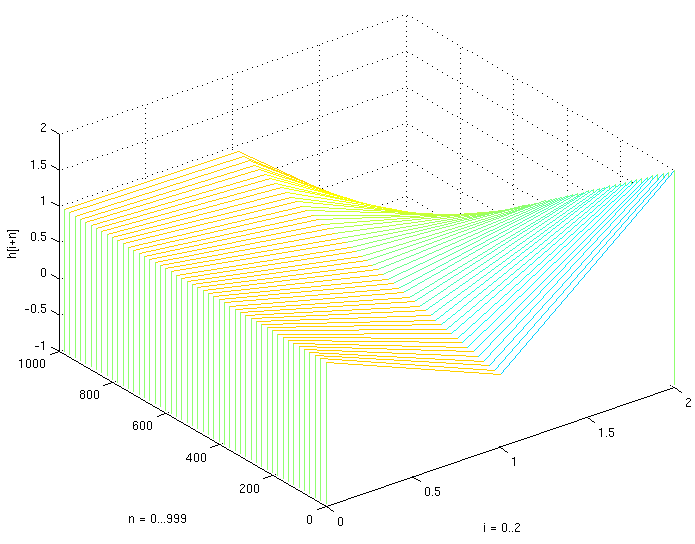
\includegraphics[width=16cm]{./plots/waterfall.png}
 % waterfall.png: 1400x920 pixel, 90dpi, 39.51x25.97 cm, bb=0 0 1120 736
 \caption{Wasserfall Darstellung der Impulsantwort}
 \label{fig:waterfall}
\end{figure}

\subsection{(c) Adaptiver Filter ohne Rauschen}

In der Abbildung \ref{fig:c_20} bzw. \ref{fig:c_50} wurden die Koeffizienten
des ``unbekannten'' Systems mit den Koeffizienten des Adaptiven Systems verglichen.

Dabei kann man erkennen, dass bei einem gr��erem M das unbekannte System besser angen�hert werden kann.
Die Koeffizienten haben wie in den Abbildungen ersichtlich eine kleinere Varianz. Das ganze ist nat�rlich
logisch, da l�ngere Bl�cke verarbeitet werden.

Nachteil eines gr��eren M ist ein etwas gr��erer Berechnungsaufwand.
Ein weiterer Nachteil welcher zwar hier nicht ersichtlich ist, dass die Filterkoeffizienten
bei schnelleren �nderungen von $\textbf{h}[n]$ nicht mitkommen.

\subsection{(d) Adaptiver Filter mit Wei�em Rauschen}
In den Abbildungen \ref{fig:d_20} bzw. \ref{fig:d_50} ist zu erkennen, dass das Hinzuf�gen von
Wei�em Rauschen keinen wesentlichen Unterschied bringt. Die Abweichung von den idealen
Koeffizienten ist nat�rlich etwas gr��er.

\subsection{(e) Adaptiver Filter mit vom Eingang abh�ngigem $\nu[n]$}
In den Abbildungen \ref{fig:e_20} bzw. \ref{fig:e_50} ist zu erkennen,
dass die durch das Adaptive Filter angen�herten Koeffizienten einen Offset zu den idealen Koeffizienten haben.
Dies liegt daran, dass $\nu[n]$ abh�ngig vom Eingang $x[n]$ ist.

Betrachtet man die Gleichung:
\begin{equation}
 \nu[n] = 1/2 \cdot (x[n] + x[n-1])
\end{equation}

so f�llt auf, dass $\nu[n]$ aus einem Filter mit den Koeffizienten $[0.5;0.5;0]$ aus $x[n]$ erzeugt werden kann.
Dies spiegelt sich auch in den Koeffizienten des Adpativen Filters wieder. Somit l�sst sich der
``Offset'' der Koeffizienten in den Abbildungen \ref{fig:e_20} bzw. \ref{fig:e_50} erkl�ren.







\newpage

\begin{figure}[ht!]
 \centering
 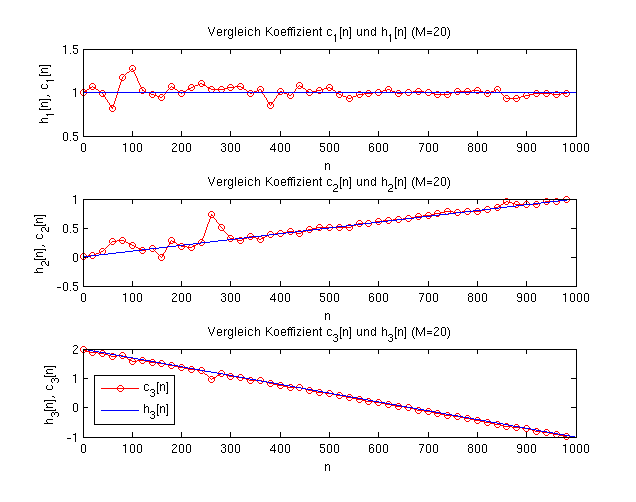
\includegraphics[width=13.5cm]{./plots/c_coefficients_M20.png}
 % waterfall.png: 1400x920 pixel, 90dpi, 39.51x25.97 cm, bb=0 0 1120 736
 \caption{Koeffizienten des Filters mit M=20, $v[n] = 0$}
 \label{fig:c_20}
\end{figure}

\begin{figure}[ht!]
 \centering
 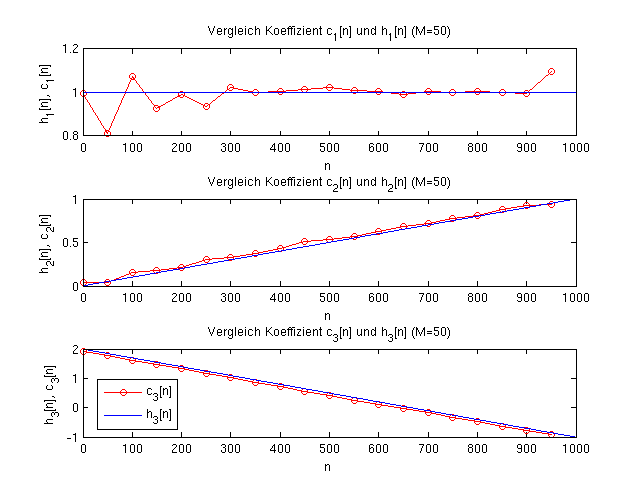
\includegraphics[width=13.5cm]{./plots/c_coefficients_M50.png}
 % waterfall.png: 1400x920 pixel, 90dpi, 39.51x25.97 cm, bb=0 0 1120 736
 \caption{Koeffizienten des Filters mit M=50, $v[n] = 0$}
 \label{fig:c_50}
\end{figure}


\begin{figure}[ht!]
 \centering
 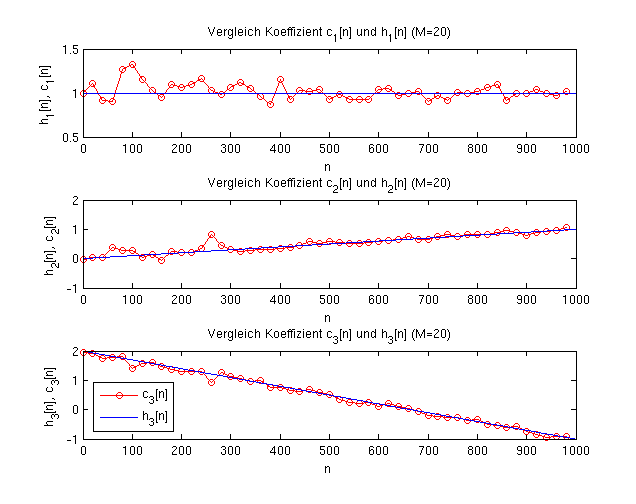
\includegraphics[width=13.5cm]{./plots/d_coefficients_M20.png}
 % waterfall.png: 1400x920 pixel, 90dpi, 39.51x25.97 cm, bb=0 0 1120 736
 \caption{Koeffizienten des Filters mit M=20, $v[n] = $ zero mean white noise with Variance = 0.5}
 \label{fig:d_20}
\end{figure}

\begin{figure}[ht!]
 \centering
 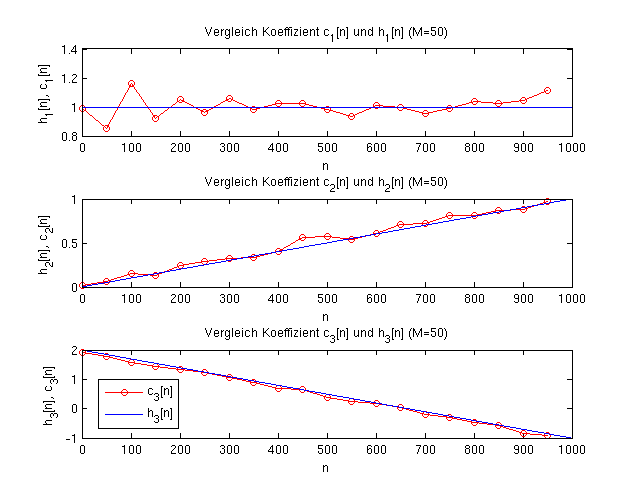
\includegraphics[width=13.5cm]{./plots/d_coefficients_M50.png}
 % waterfall.png: 1400x920 pixel, 90dpi, 39.51x25.97 cm, bb=0 0 1120 736
 \caption{Koeffizienten des Filters mit M=50, $v[n] = $ zero mean white noise with Variance = 0.5}
 \label{fig:d_50}
\end{figure}

\begin{figure}[ht!]
 \centering
 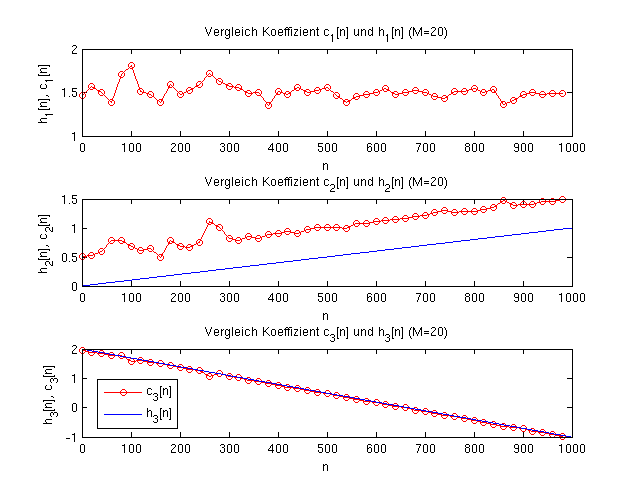
\includegraphics[width=13.5cm]{./plots/e_coefficients_M20.png}
 % waterfall.png: 1400x920 pixel, 90dpi, 39.51x25.97 cm, bb=0 0 1120 736
 \caption{Koeffizienten des Filters mit M=20, $v[n] = 0.5\cdot (x[n] + x[n-1]$}
 \label{fig:e_20}
\end{figure}

\begin{figure}[ht!]
 \centering
 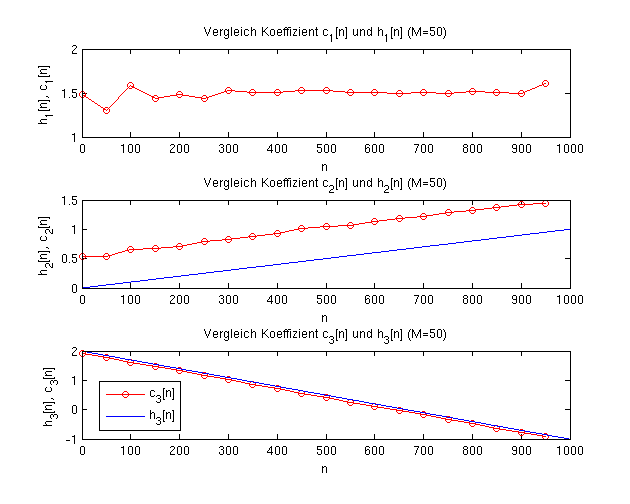
\includegraphics[width=13.5cm]{./plots/e_coefficients_M50.png}
 % waterfall.png: 1400x920 pixel, 90dpi, 39.51x25.97 cm, bb=0 0 1120 736
 \caption{Koeffizienten des Filters mit M=50, $v[n] = 0.5\cdot (x[n] + x[n-1]$}
 \label{fig:e_50}
\end{figure}


\newpage

\chapter{Listings}

\section{LS-Filter}
\lstinputlisting[language=matlab]{../matlab/ls_filter.m}

\section{Unknown System}
\lstinputlisting[language=matlab]{../matlab/unknownsystem.m}

\section{Gesamtskript 13}
\lstinputlisting[language=matlab]{../matlab/m13.m}


\section{Skript zum Berechnen und Plotten der Koeffizienten}
\lstinputlisting[language=matlab]{../matlab/calc_c_and_plot.m}


% **************************************************************************************************
% **************************************************************************************************

%\appendix
%\bibliographystyle{/.base/ieeetran}
%\bibliography{_bibliography}

% place all floats and create label on last page
\FloatBarrier\label{end-of-document}
\end{document}

